\documentclass[dvipsnames, tikz]{standalone}
\usepackage{amsmath}
\usepackage{arevmath}
\usepackage{xcolor}
\usepackage{tikz}
\usetikzlibrary{calc}
\usetikzlibrary{decorations.pathreplacing,calligraphy,3d}
\usetikzlibrary{matrix,shapes,fit,backgrounds}

\tikzset{main/.style={draw=black, line width=10pt, circle}}

\begin{document}
	\begin{tikzpicture}
		\clip (-15.5,-0.2) rectangle (15.5,6.2);
		\draw[main] (0,0) --++ (0,1);
	\end{tikzpicture}
	
	\begin{tikzpicture}
		\clip (-15.5,-0.2) rectangle (15.5,6.2);
		\draw[main] (-1,0) --++ (0,1);
		\draw[main] (0,0) --++ (0,1);
		\draw[main] (0,1.25) --++ (0,1);
		\draw[main] (1,0) --++ (0,1);
	\end{tikzpicture}

	\begin{tikzpicture}
		\clip (-15.5,-0.2) rectangle (15.5,6.2);
		\draw[main] (-3,0) --++ (0,1);
		\draw[main] (-2,0) --++ (0,1);
		\draw[main] (-2,1.25) --++ (0,1);
		\draw[main] (-1,0) --++ (0,1);
		\draw[main] (0,0) --++ (0,1);
		\draw[main] (0,1.25) --++ (0,1);
		\draw[main] (0,2.5) --++ (0,1);
		\draw[main] (1,0) --++ (0,1);
		\draw[main] (2,0) --++ (0,1);
		\draw[main] (2,1.25) --++ (0,1);
		\draw[main] (3,0) --++ (0,1);
	\end{tikzpicture}

	
\begin{tikzpicture}
		\clip (-15.5,-0.2) rectangle (15.5,6.2);
		\draw[main] (-7,0) --++ (0,1);
		\draw[main] (-6,0) --++ (0,1);
		\draw[main] (-6,1.25) --++ (0,1);
		\draw[main] (-5,0) --++ (0,1);
		\draw[main] (-4,0) --++ (0,1);
		\draw[main] (-4,1.25) --++ (0,1);
		\draw[main] (-4,2.5) --++ (0,1);
		\draw[main] (-3,0) --++ (0,1);
		\draw[main] (-2,0) --++ (0,1);
		\draw[main] (-2,1.25) --++ (0,1);
		\draw[main] (-1,0) --++ (0,1);
		
		\draw[main] (0,0) --++ (0,1);
		\draw[main] (0,1.25) --++ (0,1);
		\draw[main] (0,2.5) --++ (0,1);
		\draw[main] (0,3.75) --++ (0,1);
		
		\draw[main] (1,0) --++ (0,1);
		\draw[main] (2,0) --++ (0,1);
		\draw[main] (2,1.25) --++ (0,1);
		\draw[main] (3,0) --++ (0,1);
		\draw[main] (4,0) --++ (0,1);
		\draw[main] (4,1.25) --++ (0,1);
		\draw[main] (4,2.5) --++ (0,1);
		\draw[main] (5,0) --++ (0,1);
		\draw[main] (6,0) --++ (0,1);
		\draw[main] (6,1.25) --++ (0,1);
		\draw[main] (7,0) --++ (0,1);
	\end{tikzpicture}

	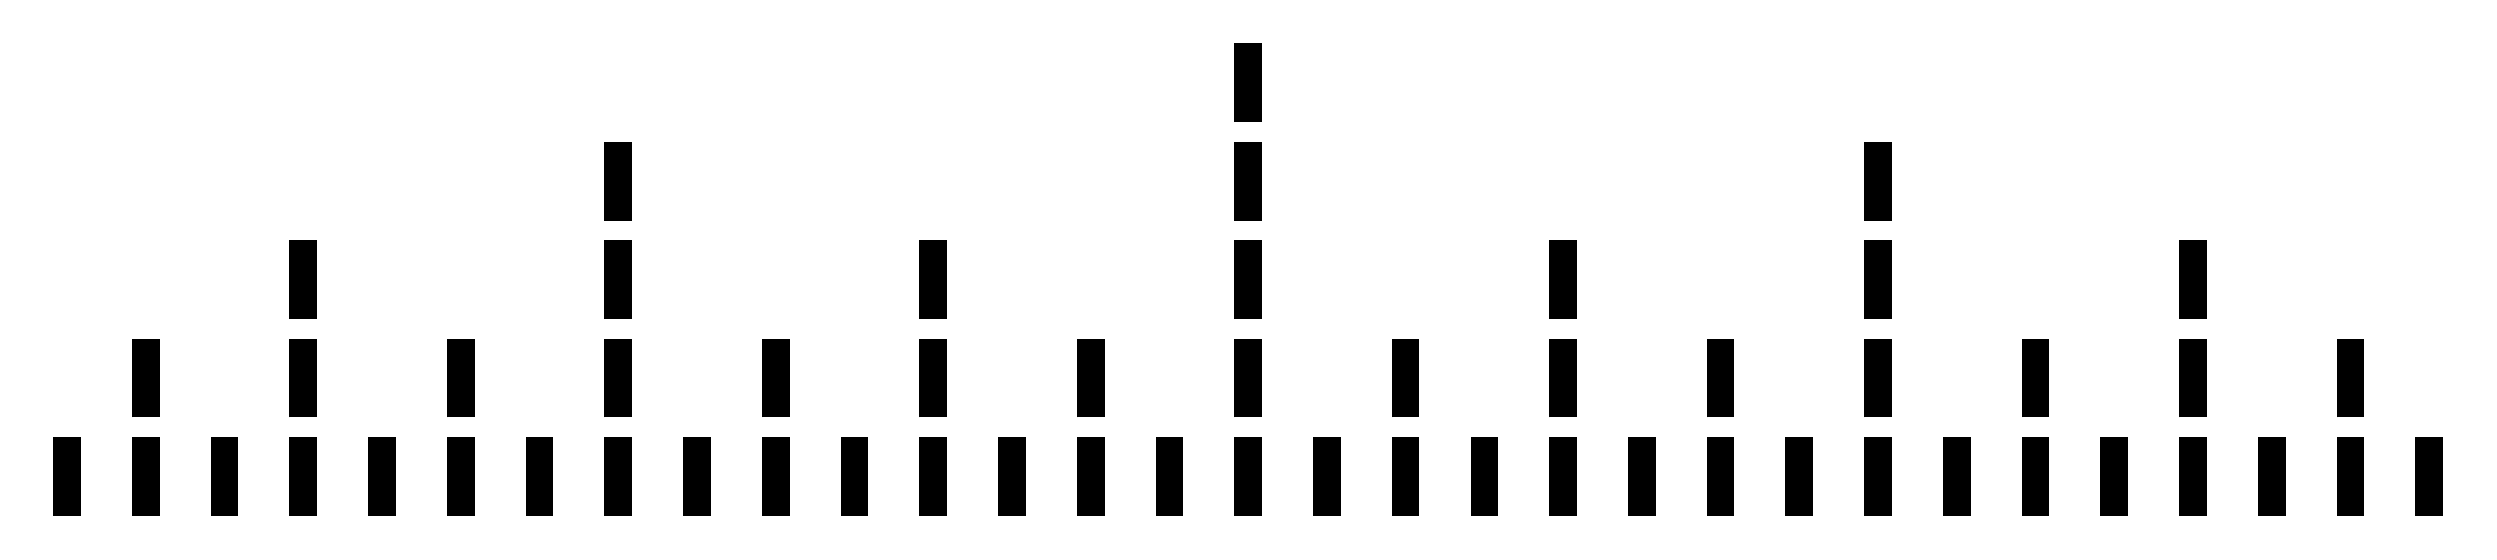
\begin{tikzpicture}
		\clip (-15.5,-0.2) rectangle (15.5,6.2);
		\begin{scope}[xshift=-8cm]
			\draw[main] (-7,0) --++ (0,1);
			\draw[main] (-6,0) --++ (0,1);
			\draw[main] (-6,1.25) --++ (0,1);
			\draw[main] (-5,0) --++ (0,1);
			\draw[main] (-4,0) --++ (0,1);
			\draw[main] (-4,1.25) --++ (0,1);
			\draw[main] (-4,2.5) --++ (0,1);
			\draw[main] (-3,0) --++ (0,1);
			\draw[main] (-2,0) --++ (0,1);
			\draw[main] (-2,1.25) --++ (0,1);
			\draw[main] (-1,0) --++ (0,1);
			
			\draw[main] (0,0) --++ (0,1);
			\draw[main] (0,1.25) --++ (0,1);
			\draw[main] (0,2.5) --++ (0,1);
			\draw[main] (0,3.75) --++ (0,1);
			
			\draw[main] (1,0) --++ (0,1);
			\draw[main] (2,0) --++ (0,1);
			\draw[main] (2,1.25) --++ (0,1);
			\draw[main] (3,0) --++ (0,1);
			\draw[main] (4,0) --++ (0,1);
			\draw[main] (4,1.25) --++ (0,1);
			\draw[main] (4,2.5) --++ (0,1);
			\draw[main] (5,0) --++ (0,1);
			\draw[main] (6,0) --++ (0,1);
			\draw[main] (6,1.25) --++ (0,1);
			\draw[main] (7,0) --++ (0,1);
		\end{scope}
		\draw[main] (0,0) --++ (0,1);
		\draw[main] (0,1.25) --++ (0,1);
		\draw[main] (0,2.5) --++ (0,1);
		\draw[main] (0,3.75) --++ (0,1);
		\draw[main] (0,5) --++ (0,1);
	
		\begin{scope}[xshift=8cm]
			\draw[main] (-7,0) --++ (0,1);
			\draw[main] (-6,0) --++ (0,1);
			\draw[main] (-6,1.25) --++ (0,1);
			\draw[main] (-5,0) --++ (0,1);
			\draw[main] (-4,0) --++ (0,1);
			\draw[main] (-4,1.25) --++ (0,1);
			\draw[main] (-4,2.5) --++ (0,1);
			\draw[main] (-3,0) --++ (0,1);
			\draw[main] (-2,0) --++ (0,1);
			\draw[main] (-2,1.25) --++ (0,1);
			\draw[main] (-1,0) --++ (0,1);
			
			\draw[main] (0,0) --++ (0,1);
			\draw[main] (0,1.25) --++ (0,1);
			\draw[main] (0,2.5) --++ (0,1);
			\draw[main] (0,3.75) --++ (0,1);
			
			\draw[main] (1,0) --++ (0,1);
			\draw[main] (2,0) --++ (0,1);
			\draw[main] (2,1.25) --++ (0,1);
			\draw[main] (3,0) --++ (0,1);
			\draw[main] (4,0) --++ (0,1);
			\draw[main] (4,1.25) --++ (0,1);
			\draw[main] (4,2.5) --++ (0,1);
			\draw[main] (5,0) --++ (0,1);
			\draw[main] (6,0) --++ (0,1);
			\draw[main] (6,1.25) --++ (0,1);
			\draw[main] (7,0) --++ (0,1);
		\end{scope}
	\end{tikzpicture}
\end{document}